\chapter{Clustering}

In order to make predictions on when a bike will arrive we will need to have a concept of hotspots where the bikes are the most.

We need to group our gps points into clusters that represent these hotspots of activity.

A technique for making these divisions is called clustering.
This section will describe the concepts of clustering as well as the possible algorithms as described in \citet{pang2006introduction}

\section{Cluster Analysis}
Cluster analysis is a technique used to group data objects based only on the information the data itself contains.
The requirement for membership in a certain cluster is often vague, as several acceptable clusterings can be made on the same dataset.
An example of this can be seen on \cref{clusterings} where the same dataset has been clustered in three radically different ways, even though all three could be regarded as correct, depending on the purpose of the clustering.

The definition of a cluster therefore depends on the dataset and the purpose of the clustering 

\begin{figure}[H]
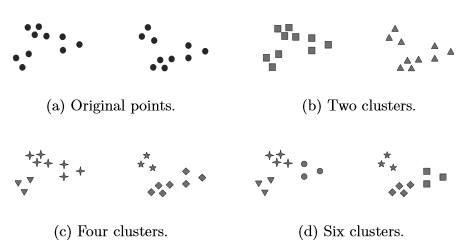
\includegraphics[width=0.5\textwidth]{graphics/clusterings}
\label{clusterings}
\caption{Different clusterings on the same dataset. From \citet{pang2006introduction}}
\end{figure}

\section{Types of clusterings}

A clustering is a collection of clusters.
This section will introduce the terminology used to describe clusterings. 

\paragraph{Hierarchical versus partitional}
A \textit{partitional clustering} is a division of data into non-overlapping subsets, where each object is in exactly one subset.
If clusters are allowed to have subclusters, the clustering is said to be \textit{hierarchical}.
A hierarchical clustering is represented as a set of nested clusters organized as a tree where each node is the union of its children.

\paragraph{Exclusive, overlapping and fuzzy clusterings}

A clustering is \textit{exclusive} if an object is assigned to exactly one cluster.
If an object can belong to more than one group the clustering is \textit{overlapping}.
If a weight is used to describe the membership of sets the clustering is said to be \textit{fuzzy}.

\paragraph{Complete versus partial}

A \textit{complete} clustering has every object assigned to a cluster while a \textit{partial} clustering can have outliers that do not belong to any cluster.

\section{Types of clusters}
The idea of a cluster depend very much on the data set it is applied on.
In this section the different notions of a cluster will be presented

\paragraph{Well separated}
A cluster is a set of objects where the objects that are similar are grouped in a cluster. 
Sometimes a threshold is used to define a minimum similarity. 
All objects in a cluster needs to be at least as similar to the other objects in a cluster for an object to be in the cluster.

\paragraph{Prototype based}
An object is placed in clusters based on prototypes that defines the clusters.
An object is placed in the cluster where the object is more similar to the prototype of the cluster than to the prototype of any other cluster.

These prototypes can be either the average value of a cluster or the most representative object of a cluster.

\paragraph{Graph based}
If the data can be represented as a graph with the objects as nodes, clusters can be defined as connected components in the graph.

\paragraph{Density based}
A cluster is defined by the density of the data objects.
A cluster is a dense region surrounded by a low density region.

\section{Techniques}

This section will explore the techniques that exist in cluster analysis.

\subsection{K-means}

K-means is a technique that creates a partitioning from prototypes where the prototypes are the center of the clusters.

The basic algorithm takes a number K and generates K initial center points.
Each data object is then assigned to the nearest center point.
The center points are now updated to be the center of the created clusters.
These steps are repeated until no point changes cluster or the center points do not change.
The algorithm is described as pseudo code in \cref{kmeans-algo}

\begin{algorithm}
\SetAlgoLined
\SetKwInOut{Input}{input}\SetKwInOut{Output}{output}
\Input{An integer k, the number of desired clusters}
\Output{An assigment of each point to a cluster}

select K initial center points \\
\Repeat{Center points do not change\label{repeatcondition}} {
Form K clusters by assigning each point to the closest center point \\
Calculate the centerpoint of the newly formed clusters \label{recalculate}\\
}
\caption{The K-means clustering algorithm}\label{kmeans-algo}
\end{algorithm}

Because most of the convergence happens in the initial iterations the condition in \cref{repeatcondition} can be replaced by a weaker condition, like repeat until only 1\% of the points change clusters.

\paragraph{Assignment of points} The assignment of points to cluster differ depending on the data.
If the data is in the Euclidean space Euclidean distance may be appropriate, while other data types will be to use another similarity measure.

\paragraph{Calculate center points} In \cref{recalculate} of the algorithm it is stated that it needs to ``Calculate the center point of the newly formed clusters''. 
This statement is very general in the sense that it depends on the data, and even on a particular type of data it can be done in different ways.
Again considering Euclidean space data points, the quality of a selected center point can be measured by the Sum of Squared Errors (SSE) of the distance to the center point of each data point.
In this way it is preferred to choose a clustering with the lowest SSE value.

\paragraph{Choosing initial center points}
The selection of the initial center points are very important because poor initial center points risk producing a local minimum instead of the global minimum, and thus a suboptimal clustering.

The easiest approach, but also the one with the highest risk of producing poor results, is randomly generated points. 
An improvement to this approach is to generate more than one set of initial points and choosing the set with the lowest SSE value. 

Another more refined way of choosing initial center point is to take a sample of the points and perform a hierarchical clustering algorithm of this subset.
K clusters can then be extracted from the hierarchical clustering and their centers are found.

A third method is to take one random point and then selecting the point farthest away from all selected points until K points are selected.
This method ensures that the points are separated, but risk choosing outliers that do not represent any cluster.

\paragraph{Strengths and weaknesses}
the K-means algorithm can have some difficulty finding clusters where the data is placed in shapes very different from globular. 
Also very big differences in size of cluster may make it difficult for K-means to differentiate the clusters.


\stefan{The following topics are covered in the book and can be included if we find it necessary: Complexity, Additional issues, Bisecting K-means (an extension of Kmeans)}

\subsection{Hierarchical Clustering}

Hierarchical clustering arranges the points in a hierarchy depending on the distance between points.
Hierarchical clustering can be performed either by starting at the top of the tree or at the bottom.
\textit{Agglomerative hierarchical clustering} starts by considering all points as being in an individual cluster and generating the hierarchy by merging the closest clusters. 
\textit{Divisive hierarchical clustering} start by considering all points as being in a single cluster and then splitting the clusters at each step.

This section will focus on the agglomerative variant of hierarchical clustering algorithms.
As just described agglomerative hierarchical clustering starts with individual clusters and merges them at each step.
This is expressed as an algorithm in \cref{agglo-hier}.

\begin{algorithm}
\SetAlgoLined
\SetKwInOut{Input}{input}\SetKwInOut{Output}{output}
\Output{A tree defining the hierarchies of the clustering}

Compute the proximity matrix\\
\Repeat{Only one cluster is remaining}{
Merge the closest two clusters\\
Update the proximity matrix to reflect the proximity between the newly created cluster and the old clusters\\
}
\caption{Agglomerative hierarchical clustering algorithm clustering}\label{agglo-hier}
\end{algorithm}

\paragraph{Defining proximity}
The key to the agglomerative hierarchical clustering algorithm is to choose a fitting measure for proximity.
An approach is to look at the clusters as a graph.
Then clusters can be compared by looking at either the distance between the closest members of the clusters, or the distance between the farthest members of the clusters.
Another method is to look at the increase in SSE to the center of a cluster when performing a merge, and minimizing this value.
This method is called Ward's method.

\stefan{The following is covered in the book and can be added if we find it necessary: Complexity, proximity examples, Key issues}

\subsection{DBSCAN}
DBSCAN in a densitybased clusteringalgorithm that locates regions of high density that are separated by regions of low density.

\paragraph{Center based point density}
As with similarity there exists different methods of determining density.
One approach is to use a point as a center and calculate the number of point that are within a certatin radius of the point.
Using this measure it can be classified whether a point is placed in a dense region (a core point),at the edge of a dense region (a border point) or is in a region with sparse density (a noise point).
The exact definition of the three types of points are as follows:

\textbf{Core point} These points have at least $ MinPts $ points in a radius of $ eps $ from it. 
Here $ MinPts $ is the number of points in the vicinity of a point regarded as dense by the user, and $ eps $ is the radius to look for these points.
\textbf{Border points} A point that is not a core point, but is in the neighbourhood of a core point. 
One point can be a border point to several core points.
\textbf{Noise point} Any point that is neither a core point or a border point.

Given these definitions, the algorithm is described in \cref{dbscan-algo}

\begin{algorithm}
Label all points as core point, border point or noise point \\
Eliminate all noise points \\
Put an edge between core points that are within $ eps $ of each other \\
Make each group of core points that are connected into a cluster \\
Assign each border point to one of the clusters associated with the border point. 
\caption{The DBSCAN clustering algorithm}\label{dbscan-algo}
\end{algorithm}

\stefan{expand on dbscan}